% SQLAlchemy clever abstraction class to DB backend
%
% Author  : Gregory DAVID
%
% Don’t forget that page size is 12,8cm x 9,6cm, when sizing images
% for example.
%%

\documentclass[english]{beamer}

\usepackage{babel}
\usepackage{layout}
\usepackage{glossaire}
\newcommand{\PROGRAMDIR}{data}
\usepackage[hide=true,dir=\PROGRAMDIR]{bashful}
\lstdefinestyle{bashfulScript}{basicstyle=\tiny\ttfamily,emptylines=1,numbers=left,language={}}
\lstdefinestyle{bashfulStdout}{basicstyle=\tiny\ttfamily,emptylines=1,numbers=right,language={}}

\usetheme{Warsaw}
\usecolortheme{crane}
\useinnertheme{circles}
\newcommand{\MYTITLE}{\gls{SQLALCHEMY}}
\newcommand{\MYSUBTITLE}{how to start using the clever abstraction class}
\newcommand{\INSTITUTE}{P1~Security}

\title{\MYTITLE}
\subtitle{\MYSUBTITLE}
\author[\gitAuthorIsoDate, \REVISIONS, \INSTITUTE]{\ME}
\institute{\INSTITUTE}
\date{\today}

\begin{document}
\maketitle

\begin{frame}
    \frametitle{Agenda}
    \tableofcontents
\end{frame}

\section{Context}
\begin{frame}
    \tableofcontents[current]
\end{frame}

\subsection{Data persistency}
\begin{frame}
    \frametitle{\gls{SQLITE} example}
    \lstset{basicstyle=\tiny\ttfamily,language=Python,numbers=left}
    \lstinputlisting{\PROGRAMDIR/sqlite_example.py}
\end{frame}
\begin{frame}[containsverbatim]
    \frametitle{\gls{SQLITE} example}
    \begin{description}
    \item[Output] ~\\
\bash[stdout,ignoreExitCode,ignoreStderr,prefix={}]
rm sqlite.db
./sqlite_example.py
\END
    \item[File type] ~\\
\bash[stdout,ignoreExitCode,ignoreStderr,prefix={}]
file ./sqlite.db
\END
    \end{description}
\end{frame}

\subsection{Data concurrency}
\begin{frame}[containsverbatim]
    \frametitle{\gls{MARIADB} example}
    \lstset{basicstyle=\tiny\ttfamily,language=Python,numbers=left}
    \lstinputlisting{\PROGRAMDIR/mariadb_example.py}
\end{frame}
\begin{frame}[containsverbatim]
    \frametitle{\gls{MARIADB} example}
    \begin{description}
    \item[Output] ~\\
\bash[ignoreExitCode,ignoreStderr,prefix={}]
make clean-mariadb
\END
\bash[stdout,ignoreExitCode,ignoreStderr,prefix={}]
./mariadb_example.py
\END
    \end{description}
\end{frame}

\subsection{What about data storage switching?}
\begin{frame}
    \begin{itemize}
    \item Unit testing environment is not a favorable context to deploy the
        complexity of data concurrency.
    \item \href{https://peps.python.org/pep-0249/}{Python Database API
            Specification v2.0 \texttt{PEP 249}} is about to encourage
        similarity between the Python modules that are used to access
        databases.
    \item Database backends do not implement standard \gls{SQL}
    \end{itemize}
\end{frame}
\begin{frame}[containsverbatim]
    What a pity to maintain two code flavors!
    \bash[ignoreExitCode,ignoreStderr,prefix={}]
diff -u sqlite_example.py mariadb_example.py
\END
    \lstset{basicstyle=\scriptsize\ttfamily,language=diff,numbers=none}
    \begin{center}
        \resizebox{\textwidth}{!}{%
            \lstinputlisting{\PROGRAMDIR/\jobname.stdout}
        }
    \end{center}
\end{frame}

\section{Using \gls{SQLALCHEMY}}
\begin{frame}
    \tableofcontents[current]
\end{frame}
\begin{frame}
    Always refer to \gls{SQLALCHEMY} documentation
    \url{https://docs.sqlalchemy.org/}
\end{frame}
\begin{frame}
    \begin{center}
        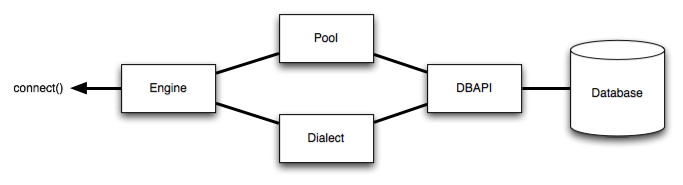
\includegraphics[width=0.75\textwidth]{data/sqla_engine_arch.png}
    \end{center}
\end{frame}

\subsection{Installation}
\begin{frame}[containsverbatim]
    \frametitle{PyPi package repository}
    \lstset{basicstyle=\tiny\ttfamily,language=sh,numbers=left}
    \lstinputlisting{\PROGRAMDIR/install_pip.sh}
    See \url{https://pypi.org/project/SQLAlchemy/}
\end{frame}

\subsection{\gls{ORM}}
\begin{frame}[containsverbatim]
    \frametitle{Getting started}
    \lstset{basicstyle=\tiny\ttfamily,language=Python,numbers=left}
    \lstinputlisting[linerange=2-8]{\PROGRAMDIR/summary_example.py}
\end{frame}
\begin{frame}[containsverbatim]
    \frametitle{Modeling}
    \lstset{basicstyle=\tiny\ttfamily,language=Python,numbers=left}
    \lstinputlisting[linerange=10-17]{\PROGRAMDIR/summary_example.py}
\end{frame}

\subsection{Implement a DB agnostic code}
\begin{frame}
    \frametitle{The \texttt{sqlalchemy.Session} object}
    \begin{itemize}
    \item In the most general sense, the \texttt{Session} establishes
        all conversations with the database and represents a
        \emph{holding zone} for all the objects which you've loaded or
        associated with it during its lifespan.
    \item It provides the interface where \texttt{SELECT} and other
        queries are made that will return and modify \gls{ORM}-mapped
        objects.
    \end{itemize}
\end{frame}
\begin{frame}
    \lstset{basicstyle=\tiny\ttfamily,language=Python,numbers=left}
    \lstinputlisting[linerange=19-34]{\PROGRAMDIR/summary_example.py}
\end{frame}

\subsection{All together}
\begin{frame}[containsverbatim]
    \lstset{basicstyle=\tiny\ttfamily,language=Python,numbers=left}
    \resizebox{\textwidth}{!}{%
        \lstinputlisting[emptylines=*0]{\PROGRAMDIR/summary_example.py}
    }
\end{frame}
\begin{frame}[containsverbatim]
    \frametitle{Output}
\bash[stdout,ignoreExitCode,ignoreStderr,prefix={}]
./summary_example.py
\END
\end{frame}

\subsection{Ease of DB switching}
\begin{frame}[containsverbatim]
    \frametitle{From \gls{SQLITE} to \gls{MARIADB}}
    \lstset{basicstyle=\tiny\ttfamily,language=Python,numbers=left}
    \bash[ignoreExitCode,ignoreStderr,prefix={}]
diff -u summary_example.py mariadb_summary_example.py
\END
    \lstset{basicstyle=\scriptsize\ttfamily,language=diff,numbers=none}
    \resizebox{\textwidth}{!}{%
        \lstinputlisting{\PROGRAMDIR/\jobname.stdout}
    }
\end{frame}

\section{Need documentation?}
\begin{frame}
    \begin{itemize}
    \item \href{https://docs.sqlalchemy.org/}{Main \gls{SQLALCHEMY} documentation}
    \item \href{https://docs.sqlalchemy.org/en/20/orm/declarative_mapping.html}{\gls{SQLALCHEMY} \texttt{Mapping Classes with Declarative}}
    \item \href{https://docs.sqlalchemy.org/en/20/core/types.html}{\gls{SQLALCHEMY} \texttt{SQL Datatype Objects}}
    \item \href{https://docs.sqlalchemy.org/en/20/orm/relationships.html}{\gls{SQLALCHEMY} \texttt{Relationship Configuration}}
    \item \href{https://docs.sqlalchemy.org/en/20/orm/session.html}{Using the \gls{SQLALCHEMY} \texttt{Session}}
    \item \href{https://docs.sqlalchemy.org/en/20/orm/queryguide/}{\gls{SQLALCHEMY} \texttt{Querying guide}}
    \end{itemize}
\end{frame}

\clearpage
{\scriptsize\printglossary}
\end{document}
